\documentclass{beamer}

\usetheme{Padova}

\title{Esame di Laurea in Informatica}
\subtitle{Implementazione di modelli di programmazione matematica per problemi di bin packing}
\author{Daniel Rossi}
\date{18 Dicembre 2018}


\begin{document}

	\maketitle

	\begin{frame}{Outline}
		\tableofcontents
	\end{frame}

	\section{Introduction}

	\begin{frame}{Introduzione}
		\begin{minipage}[c]{0.45\textwidth}
			\large{\uppercase{Statistiche nazionali trasporti}} \vspace{.5em}
		\end{minipage}
			\hfill
			\begin{minipage}[c]{0.45\textwidth}
				
\includegraphics[width=\textwidth]{figures/logo}
			\end{minipage}
			\begin{block}{Logistica}
				7\% del PIL italiano
			\end{block}
			\begin{block}{Costi}
				11\% maggiore rispetto partner europei
			\end{block}
	\end{frame}


	\section{First section}

	\begin{frame}{First section}
		\begin{block}{Normal block}
			Fusce luctus venenatis felis quis semper
		\end{block}

		\begin{alertblock}{Modello matematico}
			$$ max\; z = f ( x )\;\; (oppure\; min\; z = f ( x ))$$
			s.t.
			$$g_i (x) = \begin{cases} \leq b_i \\ = b_i, & i = 1,\dots,m \\ \geq b_i \end{cases}$$
			$$x = (x_1,\dots,x_n) \in X \subseteq \mathbb{R}^n$$
		\end{alertblock}

		\begin{exampleblock}{Example block}
			Proin tincidunt, neque at tincidunt mollis
		\end{exampleblock}
	\end{frame}
	
	\section{Second section}
		\begin{frame}{Second section}
			$$ max\; z = f ( x )\;\; (oppure\; min\; z = f ( x ))$$
			s.t.
			$$g_i (x) = \begin{cases} \leq b_i \\ = b_i, & i = 1,\dots,m \\ \geq b_i \end{cases}$$
			$$x = (x_1,\dots,x_n) \in X \subseteq \mathbb{R}^n$$
		\end{frame}
	\section{Ciucia}
		\begin{frame}{ciucia}
			\begin{figure}[H]
				\begin{center} 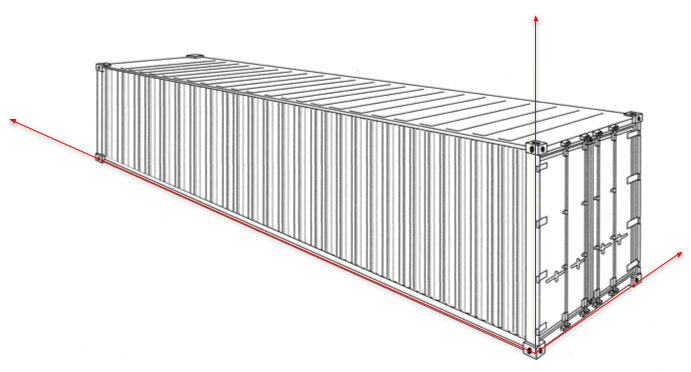
\includegraphics[scale=0.4]{figures/container_arrows}
				\end{center}
			\end{figure}
		\end{frame}{ciucia}

\end{document}
